\chapter{Graph Isomorphism e la gerarchia di Weisfeiler--Leman}

% ---------------------------------------------------------------------------
% Nel quaderno il capitolo si apre a metà di p.79, con il titolo sottolineato
% «Graph Isomorphism»; accanto, fra parentesi, un nome proprio di lettura
% incerta («Francesco Nassimbeni»), verosimilmente chi ha tenuto questa parte
% del corso. Il nome non è riportato nel testo perché la lettura resta dubbia.
% ---------------------------------------------------------------------------

Le tre pagine di quaderno da cui nasce questo capitolo stanno fuori dal programma
ordinario del corso --- sono gli appunti di un seminario --- ed è per questo che le si
raccoglie in appendice. Il quaderno le lascia allo stato di traccia: titoli, formule
chiave, qualche disegno, e l'ultima pagina si interrompe a metà. Qui se ne dà una
versione leggibile, colmando le lacune con i risultati standard della letteratura;
tutte le integrazioni sono registrate nelle note editoriali.

Il problema di partenza è il \emph{graph isomorphism}: dati due grafi $G$ e $H$,
stabilire se esiste una biiezione fra i loro vertici che preservi gli archi, nel qual
caso si scrive $G \cong H$. Non se ne conosce un algoritmo polinomiale, né lo si sa
$\NP$-completo. La famiglia di test di Weisfeiler--Leman è la risposta pratica al
problema: una gerarchia di procedure polinomiali, indicizzate da un parametro $k$, che
non lo risolvono ma lo attaccano dal lato facile --- sanno certificare il \emph{non}
isomorfismo, mai l'isomorfismo --- e che diventano tanto più fini quanto più $k$ cresce.

\section{WL-1: il raffinamento dei colori}

\scan{79}

Il test di Weisfeiler--Leman di dimensione~$1$ --- il classico \emph{raffinamento dei
colori} (\emph{color refinement}) --- assegna un colore a ogni vertice e lo raffina
iterativamente: a ogni passo il nuovo colore di un vertice è determinato dal suo colore
corrente e dal multi-insieme dei colori dei suoi vicini. La colorazione partiziona
l'insieme dei vertici in classi di colore, e il procedimento si arresta quando la
partizione non si raffina più.

\begin{figure}[H]
  \centering
  % wl1-partizione-colori -- pag. 79
% Il disco e' l'insieme dei vertici V; i settori sono le classi di colore
% prodotte dal raffinamento e le crocette i vertici che vi cadono dentro.
% NB: nel quaderno la crocetta manca nel settore piu' piccolo (in alto a
% sinistra) -- quattro settori, tre crocette -- e qui la si riproduce cosi'
% com'e', come da specifica registrata nelle note editoriali.
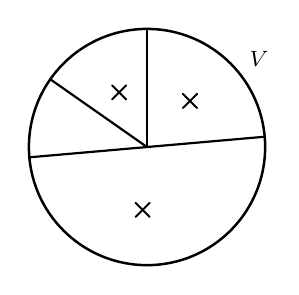
\begin{tikzpicture}[x=1cm,y=1cm,line join=round,line cap=round,font=\footnotesize]

  % ---- il disco V ----------------------------------------------------------
  \draw[line width=0.9pt] (0,0) circle (1.5);

  % ---- il diametro, leggermente inclinato ----------------------------------
  \draw[line width=0.8pt] (185:1.5) -- (5:1.5);

  % ---- i due raggi che suddividono la meta' superiore ----------------------
  \draw[line width=0.8pt] (0,0) -- (90:1.5);
  \draw[line width=0.8pt] (0,0) -- (145:1.5);

  % ---- i vertici, come nel manoscritto (tre crocette in quattro settori) ---
  \foreach \ang/\rad in {266/0.80, 47/0.80, 117/0.78}{
    \draw[line width=0.7pt]
      ([shift={(\ang:\rad)}]-0.09,-0.09) -- ([shift={(\ang:\rad)}]0.09,0.09)
      ([shift={(\ang:\rad)}]-0.09, 0.09) -- ([shift={(\ang:\rad)}]0.09,-0.09);
  }

  % ---- nome dell'insieme ---------------------------------------------------
  \node[anchor=south west,inner sep=1pt] at (38:1.60) {$V$};

\end{tikzpicture}

  \caption{Il raffinamento dei colori partiziona l'insieme dei vertici in classi di
  colore.}
  \label{fig:wl1-partizione}
\end{figure}

Il colore che WL-1 assegna a un vertice dopo $r$ raffinamenti codifica il suo
\emph{albero di srotolamento} (\emph{unrolling}) di profondità $r$: l'albero che ha per
radice il vertice, per figli della radice i suoi vicini, per figli di questi i vicini
dei vicini, e così via.

\begin{figure}[H]
  \centering
  % wl1-grafo-e-unrolling -- pag. 79
% Due pannelli: a sinistra il grafo G (un albero con due centri, sei vertici
% colorati R, B, G, N); a destra il suo srotolamento di profondita' 2 radicato
% nel vertice N.
% Controllo semantico: i figli della radice sono i vicini di N, cioe' R, B
% (foglia) e B (il secondo centro); sotto ciascuno compaiono i suoi vicini,
% compreso il ritorno al padre. Le due foglie R e B hanno il solo vicino N; il
% secondo centro B ha per vicini G, R e N.
% NB: nel quaderno i pallini non sono colorati, solo etichettati con l'iniziale
% del colore (Rosso, Blu, Giallo, Nero): si mantiene questa scelta.
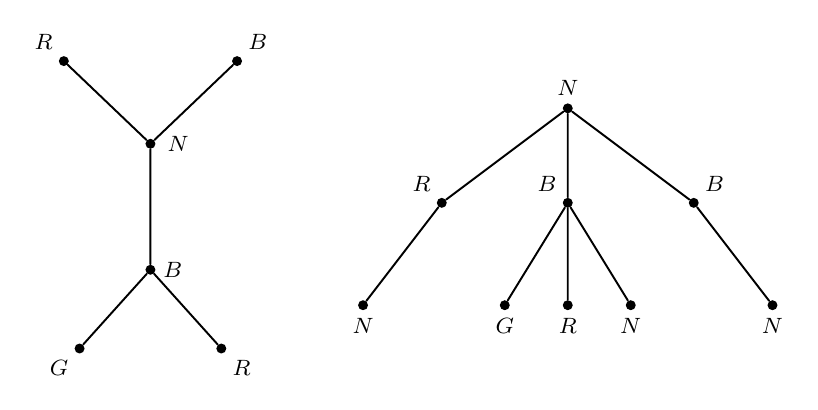
\begin{tikzpicture}[x=1cm,y=1cm,line join=round,line cap=round,font=\footnotesize,
    nodo/.style={circle,fill,inner sep=0pt,minimum size=3.6pt},
    arco/.style={line width=0.7pt},
    col/.style={inner sep=2.5pt}]

  % ======================= pannello sinistro: il grafo G ===================
  \begin{scope}[shift={(0,0)}]
    \node[nodo] (c1) at ( 0.00, 0.00) {};   % centro superiore, colore N
    \node[nodo] (r1) at (-1.10, 1.05) {};   % foglia R
    \node[nodo] (b1) at ( 1.10, 1.05) {};   % foglia B
    \node[nodo] (c2) at ( 0.00,-1.60) {};   % centro inferiore, colore B
    \node[nodo] (g)  at (-0.90,-2.60) {};   % foglia G
    \node[nodo] (r2) at ( 0.90,-2.60) {};   % foglia R

    \draw[arco] (c1) -- (r1)  (c1) -- (b1)  (c1) -- (c2)
                (c2) -- (g)   (c2) -- (r2);

    \node[col,anchor=west,inner sep=4pt] at (c1.east) {$N$};
    \node[col,anchor=south east] at (r1.north west) {$R$};
    \node[col,anchor=south west] at (b1.north east) {$B$};
    \node[col,anchor=west]       at (c2.east)       {$B$};
    \node[col,anchor=north east] at (g.south west)  {$G$};
    \node[col,anchor=north west] at (r2.south east) {$R$};
  \end{scope}

  % ============ pannello destro: lo srotolamento radicato in N =============
  \begin{scope}[shift={(5.30,0.45)}]
    \node[nodo] (t)   at ( 0.00, 0.00) {};   % radice: il vertice N
    \node[nodo] (tR)  at (-1.60,-1.20) {};   % vicino R (foglia)
    \node[nodo] (tB)  at ( 0.00,-1.20) {};   % vicino B (secondo centro)
    \node[nodo] (tB2) at ( 1.60,-1.20) {};   % vicino B (foglia)
    \node[nodo] (l1)  at (-2.60,-2.50) {};   % vicino di R: N
    \node[nodo] (l2)  at (-0.80,-2.50) {};   % vicini del secondo centro: G
    \node[nodo] (l3)  at ( 0.00,-2.50) {};   %                            R
    \node[nodo] (l4)  at ( 0.80,-2.50) {};   %                            N
    \node[nodo] (l5)  at ( 2.60,-2.50) {};   % vicino di B (foglia): N

    \draw[arco] (t) -- (tR)  (t) -- (tB)  (t) -- (tB2)
                (tR) -- (l1)
                (tB) -- (l2)  (tB) -- (l3)  (tB) -- (l4)
                (tB2) -- (l5);

    \node[col,anchor=south]      at (t.north)      {$N$};
    \node[col,anchor=south east] at (tR.north west) {$R$};
    \node[col,anchor=south east] at (tB.north west) {$B$};
    \node[col,anchor=south west] at (tB2.north east){$B$};
    \node[col,anchor=north]      at (l1.south)     {$N$};
    \node[col,anchor=north]      at (l2.south)     {$G$};
    \node[col,anchor=north]      at (l3.south)     {$R$};
    \node[col,anchor=north]      at (l4.south)     {$N$};
    \node[col,anchor=north]      at (l5.south)     {$N$};
  \end{scope}

\end{tikzpicture}

  \caption{A sinistra un grafo i cui vertici portano quattro colori distinti $R$, $B$,
  $G$, $N$; a destra l'albero di srotolamento di profondità~$2$ radicato nel vertice
  $N$.}
  \label{fig:wl1-unrolling}
\end{figure}

Per decidere l'isomorfismo di due grafi $G$ e $H$ si esegue il raffinamento su entrambi
e si confrontano i multi-insiemi dei colori finali: il test ha esito \emph{vero} quando
i due multi-insiemi coincidono. Valgono allora
\begin{align*}
  G \cong H &\;\Longrightarrow\; \mathrm{WL}\text{-}1(G,H) = \text{vero},\\
  \mathrm{WL}\text{-}1(G,H) = \text{vero} &\;\nRightarrow\; G \cong H,\\
  \mathrm{WL}\text{-}1(G,H) = \text{falso} &\;\Longrightarrow\; G \ncong H.
\end{align*}

\begin{osservazione}
  WL-1 è dunque un test con errore \emph{unilatero}: la risposta negativa è una prova di
  non isomorfismo, mentre la risposta positiva non permette di concludere nulla. La
  terza implicazione è la contronominale della prima.
\end{osservazione}

L'esempio minimale di fallimento è la coppia formata dal ciclo $C_6$ e dall'unione
disgiunta di due triangoli: entrambi i grafi sono $2$-regolari, tutti i vertici restano
dello stesso colore a ogni iterazione, e WL-1 risponde \emph{vero} pur trattandosi di
grafi non isomorfi. È questa cecità che si cerca di curare salendo di dimensione.

\section{WL-\texorpdfstring{$k$}{k}: colorare le \texorpdfstring{$k$}{k}-uple}

Il potere discriminante del test si accresce colorando non più i singoli vertici, ma le
$k$-uple di vertici: ogni $\bar v = (v_1,\dots,v_k) \in V^{k}$ viene trattata come un
unico oggetto da colorare. Servono due ingredienti --- i \emph{tipi atomici}, che danno
la colorazione iniziale, e i \emph{vicinati}, che danno il passo di raffinamento.

\subsection{Tipi atomici e colorazione iniziale}

Il colore iniziale di una $k$-upla è il suo \emph{tipo atomico}
$\operatorname{atp}(\bar v)$, cioè l'informazione puramente locale sulla $k$-upla:
quali componenti coincidono ($v_i = v_j$) e quali coppie ordinate $(v_i,v_j)$ sono archi
del grafo. In altri termini $\operatorname{atp}(\bar v)$ è il tipo di isomorfismo del
sottografo \emph{ordinato} indotto da $\bar v$: due $k$-uple $\bar v$ e $\bar v'$
partono con lo stesso colore se e solo se la corrispondenza $v_i \mapsto v_i'$,
componente per componente, è un isomorfismo fra i due sottografi indotti.

\begin{figure}[H]
  \centering
  % wlk-tipo-atomico -- pag. 79
% Il tipo atomico di una k-upla e' la sua "fotografia locale": quali componenti
% coincidono e quali coppie ordinate sono archi. Qui la tripla (u,v,w) con
% u -> v e v -> w, e nessun arco fra u e w.
% NB: nel quaderno le parentesi sono angolari e la freccia v -> w si ferma poco
% prima del pallino; qui parentesi tonde (come nel testo) e freccia che tocca
% il nodo.
\begin{tikzpicture}[x=1cm,y=1cm,line join=round,line cap=round,font=\footnotesize,
    nodo/.style={circle,fill,inner sep=0pt,minimum size=3.6pt},
    arco/.style={line width=0.8pt,-{Stealth[length=4pt,width=3pt]},shorten >=0.6pt}]

  % ---- la scritta a sinistra, come nel quaderno ----------------------------
  \node[anchor=east,inner sep=0pt] at (-0.75,0.28) {$\operatorname{atp}(u,v,w,\dots)$};

  % ---- i tre vertici della tripla -----------------------------------------
  \node[nodo] (u) at (0.00, 0.00) {};
  \node[nodo] (v) at (1.10, 0.90) {};
  \node[nodo] (w) at (1.15,-0.35) {};

  \node[anchor=south east,inner sep=2pt] at (u.north west) {$u$};
  \node[anchor=south,inner sep=2.5pt]    at (v.north)      {$v$};
  \node[anchor=west,inner sep=3pt]       at (w.east)       {$w$};

  % ---- gli archi orientati -------------------------------------------------
  \draw[arco] (u) -- (v);
  \draw[arco] (v) -- (w);

\end{tikzpicture}

  \caption{Il tipo atomico della $k$-upla $(u,v,w,\dots)$ registra le coincidenze fra le
  componenti e le adiacenze: qui $u \to v$ e $v \to w$.}
  \label{fig:wlk-tipo-atomico}
\end{figure}

\scan{80}

La colorazione iniziale è dunque
\[
  C_0^k(\bar v) \;=\; \operatorname{atp}(\bar v)
  \qquad \forall\, \bar v \in V^{k} .
\]

\begin{figure}[H]
  \centering
  % wlk-tupla -- pag. 80
% Le k componenti v_1,...,v_k sono raccolte in un unico oggetto vbar: e' a
% questo, e non ai singoli vertici, che WL-k assegna un colore.
% NB: nel quaderno i nodi in alto sono quattro (v_1..v_4) e il nodo in basso e'
% spostato verso sinistra; qui l'ultimo nodo e' etichettato v_k, con i puntini
% di sospensione, per accordarsi alla notazione del testo, e il nodo in basso
% e' centrato sotto la fila.
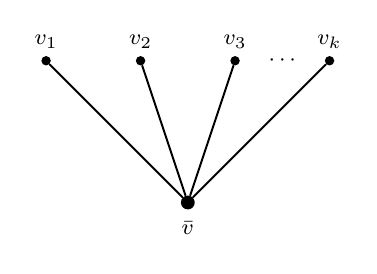
\begin{tikzpicture}[x=1cm,y=1cm,line join=round,line cap=round,font=\footnotesize,
    nodo/.style={circle,fill,inner sep=0pt,minimum size=3.4pt},
    tupla/.style={circle,fill,inner sep=0pt,minimum size=5pt},
    arco/.style={line width=0.7pt}]

  % ---- le componenti della k-upla -----------------------------------------
  \node[nodo] (v1) at (0.0,0) {};
  \node[nodo] (v2) at (1.2,0) {};
  \node[nodo] (v3) at (2.4,0) {};
  \node[nodo] (vk) at (3.6,0) {};

  \node[anchor=south,inner sep=2.5pt] at (v1.north) {$v_1$};
  \node[anchor=south,inner sep=2.5pt] at (v2.north) {$v_2$};
  \node[anchor=south,inner sep=2.5pt] at (v3.north) {$v_3$};
  \node[anchor=south,inner sep=2.5pt] at (vk.north) {$v_k$};

  \node[inner sep=1pt] at (3.0,0) {$\cdots$};

  % ---- la k-upla, vista come un solo oggetto ------------------------------
  \node[tupla] (vb) at (1.8,-1.8) {};
  \node[anchor=north,inner sep=4pt] at (vb.south) {$\bar v$};

  \draw[arco] (v1) -- (vb);
  \draw[arco] (v2) -- (vb);
  \draw[arco] (v3) -- (vb);
  \draw[arco] (vk) -- (vb);

\end{tikzpicture}

  \caption{La $k$-upla $\bar v = (v_1,\dots,v_k)$ è vista come un solo oggetto: è ad
  essa, e non ai vertici che la compongono, che WL-$k$ assegna un colore.}
  \label{fig:wlk-tupla}
\end{figure}

\subsection{Vicinati e passo di raffinamento}

I \emph{vicinati} di una $k$-upla sono le $k$-uple che si ottengono da essa sostituendo
una componente alla volta con un qualunque vertice del grafo. Scriviamo dunque
$\bar v[w/j]$ per la $k$-upla ottenuta da $\bar v$ rimpiazzando la $j$-esima componente
con $w$:
\[
  \bar v[w/j] \;=\; (v_1,\dots,v_{j-1},\,w,\,v_{j+1},\dots,v_k).
\]
Il vicinato di $\bar v$ al passo $i$ è il multi-insieme
\[
  M_i^k(\bar v) \;=\;
  \Bigl\{\!\Bigl\{\;
     \bigl( C_{i-1}^k(\bar v[w/1]),\; \dots,\; C_{i-1}^k(\bar v[w/k]) \bigr)
  \;:\; w \in V \;\Bigr\}\!\Bigr\}
\]
e il colore aggiornato è
\[
  C_i^k(\bar v) \;=\; \bigl( C_{i-1}^k(\bar v),\; M_i^k(\bar v) \bigr).
\]
Poiché il nuovo colore contiene il vecchio, ogni passo può solo raffinare la partizione
di $V^{k}$ indotta dal colore: dopo al più $n^{k}$ iterazioni --- tante quante sono le
$k$-uple --- la colorazione si stabilizza, e il test confronta i multi-insiemi dei
colori stabili dei due grafi esattamente come faceva WL-1.

\begin{esempio}[WL-2]
  Per $k = 2$ la tupla è una coppia $(u,v)$ e il vertice $w$, che scorre su tutto $V$,
  la spezza nei due «mezzi cammini» $(u,w)$ e $(w,v)$:
  \[
    M_i^2(u,v) \;=\;
    \Bigl\{\!\Bigl\{\; \bigl( C_{i-1}^2(u,w),\; C_{i-1}^2(w,v) \bigr) \;:\; w \in V
    \;\Bigr\}\!\Bigr\}.
  \]
  L'ordine delle due componenti della coppia è convenzionale --- qui è quello del
  cammino $u \to w \to v$, mentre la formula generale elenca le posizioni nell'ordine
  $1,\dots,k$ --- e basta fissarlo una volta per tutte.
\end{esempio}

\begin{figure}[H]
  \centering
  % wl2-esempio -- pag. 80
% WL-2: la coppia (u,v) viene guardata «attraverso» un terzo vertice w.
% Frecce continue = archi del grafo diretto (w->v, x->v, u->v, u->w, u->x);
% triangolo tratteggiato = le tre COPPIE in gioco nel passo di raffinamento,
% cioe' (u,v), (u,w) e (w,v).  Il tratteggio non e' un arco del grafo.
\begin{tikzpicture}[
    >=Latex,
    font=\footnotesize,
    nodo/.style={circle,fill=black,inner sep=0pt,minimum size=3.4pt},
    arco/.style={->,line width=0.7pt},
    coppia/.style={dashed,dash pattern=on 2.4pt off 1.8pt,
                   line width=0.6pt,draw=black!55},
    et/.style={font=\footnotesize,text=black!60,inner sep=1.5pt}]

  %% ---- vertici ------------------------------------------------------------
  \node[nodo,label={[inner sep=2pt]above left:$v$}]  (v) at ( 0.00, 2.00) {};
  \node[nodo,label={[inner sep=2pt]right:$w$}]       (w) at ( 2.80, 1.60) {};
  \node[nodo,label={[inner sep=3pt]below:$u$}]       (u) at ( 1.25, 0.00) {};
  \node[nodo,label={[inner sep=2pt]left:$x$}]        (x) at (-1.40,-0.10) {};

  %% ---- archi del grafo (continui, orientati) ------------------------------
  \draw[arco] (w) -- (v);
  \draw[arco] (x) -- (v);
  \draw[arco] (u) -- (v);
  \draw[arco] (u) -- (w);
  \draw[arco] (u) -- (x);

  %% ---- le tre coppie coinvolte nel passo (tratteggio, senza punte) --------
  \draw[coppia] (v) to[bend left=22]  node[et,above=1pt]           {$(w,v)$} (w);
  \draw[coppia] (w) to[bend left=22]  node[et,pos=0.45,right=1pt]  {$(u,w)$} (u);
  \draw[coppia] (v) to[bend right=18] node[et,pos=0.55,left=1pt]   {$(u,v)$} (u);

\end{tikzpicture}

  \caption{WL-2: alla coppia $(u,v)$ si guarda attraverso un terzo vertice $w$. Le
  frecce continue sono archi del grafo, il triangolo tratteggiato evidenzia le tre
  \emph{coppie} coinvolte nel passo di raffinamento: $(u,v)$, $(u,w)$ e $(w,v)$.}
  \label{fig:wl2-esempio}
\end{figure}

\subsection{FWL contro OWL}

La definizione appena data è quella \emph{folklore} (FWL): per ogni $w$ si raccoglie
un'unica $k$-upla di colori, quindi il multi-insieme ricorda \emph{quali} colori
provengono dallo stesso $w$. Nella variante \emph{oblivious} (OWL) si tengono invece
$k$ multi-insiemi separati, uno per posizione,
\[
  M_i^{k,j}(\bar v) \;=\;
  \bigl\{\!\bigl\{\, C_{i-1}^k(\bar v[w/j]) \;:\; w \in V \,\bigr\}\!\bigr\},
  \qquad j = 1,\dots,k,
\]
\[
  C_i^k(\bar v) \;=\;
  \bigl( C_{i-1}^k(\bar v),\; M_i^{k,1}(\bar v),\; \dots,\; M_i^{k,k}(\bar v) \bigr),
\]
e la correlazione fra le posizioni va perduta: FWL legge i due mezzi cammini
\emph{insieme}, per lo stesso $w$; OWL li legge \emph{separatamente}.

\begin{figure}[H]
  \centering
  % fwl-vs-owl -- pag. 80
% Trittico.  (a) configurazione di partenza: la coppia (u,v) da colorare
% (tratteggiata, come in wl2-esempio) e i due mezzi cammini u->w, w->v.
% (b) FWL: i due mezzi cammini stanno nello STESSO disegno, con un solo w:
%     il multi-insieme ricorda che i due colori vengono dallo stesso w.
% (c) OWL: i due mezzi cammini vivono in due schemi staccati, ciascuno con la
%     propria copia di w: la correlazione fra le due posizioni e' persa.
\begin{tikzpicture}[
    >=Latex,
    font=\footnotesize,
    nodo/.style={circle,fill=black,inner sep=0pt,minimum size=3.2pt},
    arco/.style={->,line width=0.7pt},
    coppia/.style={dashed,dash pattern=on 2.4pt off 1.8pt,
                   line width=0.6pt,draw=black!55},
    titolo/.style={font=\footnotesize\scshape},
    glossa/.style={font=\footnotesize,align=center,text width=3.5cm}]

  %% =================== (a) configurazione di partenza ======================
  \begin{scope}[shift={(0,0)}]
    \node[nodo,label={[inner sep=2pt]above left:$v$}] (av) at (0.00,1.45) {};
    \node[nodo,label={[inner sep=2pt]right:$w$}]      (aw) at (1.70,1.30) {};
    \node[nodo,label={[inner sep=3pt]below:$u$}]      (au) at (0.75,0.00) {};
    \draw[arco]   (aw) -- (av);
    \draw[arco]   (au) -- (aw);
    \draw[coppia] (au) -- (av);
    \node[glossa] at (0.85,-0.85) {configurazione\\di partenza};
  \end{scope}

  %% ------------------------------ separatore -------------------------------
  \draw[draw=black!25,line width=0.5pt] (2.95,-1.15) -- (2.95,2.15);

  %% ============================== (b) FWL ==================================
  \begin{scope}[shift={(3.75,0)}]
    \node[titolo] at (0.85,2.00) {FWL};
    \node[nodo,label={[inner sep=2pt]above left:$v$}] (bv) at (0.00,1.45) {};
    \node[nodo,label={[inner sep=2pt]right:$w$}]      (bw) at (1.70,1.30) {};
    \node[nodo,label={[inner sep=3pt]below:$u$}]      (bu) at (0.75,0.00) {};
    \draw[arco] (bw) -- (bv);
    \draw[arco] (bu) -- (bw);
    \node[glossa] at (0.85,-0.85) {considera la coppia:\\lo stesso $w$};
  \end{scope}

  %% ------------------------------ separatore -------------------------------
  \draw[draw=black!25,line width=0.5pt] (6.70,-1.15) -- (6.70,2.15);

  %% ============================== (c) OWL ==================================
  \begin{scope}[shift={(7.50,0)}]
    \node[titolo] at (1.05,2.00) {OWL};
    % primo mezzo cammino: w -> v
    \node[nodo,label={[inner sep=2pt]above left:$v$}] (cv)  at (0.00,1.65) {};
    \node[nodo,label={[inner sep=2pt]right:$w$}]      (cw1) at (1.00,1.20) {};
    \draw[arco] (cw1) -- (cv);
    % secondo mezzo cammino: u -> w  (copia distinta di w, schema staccato)
    \node[nodo,label={[inner sep=3pt]below:$u$}]      (cu)  at (0.85,0.00) {};
    \node[nodo,label={[inner sep=2pt]right:$w$}]      (cw2) at (1.85,0.65) {};
    \draw[arco] (cu) -- (cw2);
    \node[glossa] at (1.05,-0.85) {considera i cammini\\separatamente};
  \end{scope}

\end{tikzpicture}

  \caption{FWL contro OWL sulla coppia $(u,v)$. A sinistra la configurazione di
  partenza; al centro FWL, che considera la coppia di colori nello stesso disegno
  (stesso $w$); a destra OWL, che considera i due cammini separatamente, in due
  multi-insiemi distinti.}
  \label{fig:fwl-owl}
\end{figure}

\begin{osservazione}
  Le due varianti non hanno lo stesso potere distintivo a parità di $k$: per $k \ge 2$,
  FWL-$k$ distingue esattamente ciò che distingue OWL-$(k+1)$. La gerarchia è quindi la
  stessa, ma sfasata di uno: quando in questo capitolo si scrive WL-$k$ senza altra
  specificazione si intende la versione folklore, che è quella definita qui sopra.
\end{osservazione}

\begin{osservazione}[Il caso $k = 1$ va letto a parte]
  Presa alla lettera, la formula del passo di raffinamento è vuota per $k = 1$: si ha
  $\bar v = (v)$ e $\bar v[w/1] = (w)$, quindi
  \[
    M_i^{1}(v) \;=\; \bigl\{\!\bigl\{\, C_{i-1}^{1}(w) \;:\; w \in V \,\bigr\}\!\bigr\}
  \]
  non dipende affatto da $v$, e la colorazione non si raffina mai. È il motivo per cui
  WL-1 --- il raffinamento dei colori della sezione precedente --- si definisce a parte,
  facendo scorrere $w$ sui soli \emph{vicini} di $v$ anziché su tutto $V$. Per $k \ge 2$
  la restrizione non serve: il tipo atomico di $\bar v[w/j]$ registra già se $w$ sia o
  no adiacente alle altre componenti, e l'informazione di adiacenza non va persa.
  Vale inoltre che OWL-2 ha esattamente il potere distintivo di WL-1: convenendo che
  FWL-1 sia per definizione WL-1, lo sfasamento di uno dell'osservazione precedente si
  estende anche al primo livello, e la gerarchia comincia a essere davvero più fine da
  OWL-3, ossia da FWL-2, in poi.
\end{osservazione}

\section{Che cosa distingue WL-\texorpdfstring{$k$}{k}}

Fissato $k$, quali coppie di grafi sfuggono al test? La domanda ha tre risposte, di
natura molto diversa, ed è a queste che il quaderno dedica le ultime righe:
una \emph{combinatoria} --- su quali classi di grafi un $k$ fissato basta ---, una
\emph{algebrica} --- il rilassamento continuo dell'isomorfismo ---, e una \emph{logica}
--- il frammento del prim'ordine che ha lo stesso potere separante del test.

\subsection{Minori esclusi}

Escludere un minore fisso comporta dimensione di WL limitata: per ogni grafo $H$ esiste
un $k = k(H)$ tale che ogni grafo che non contiene $H$ come minore viene identificato da
WL-$k$, cioè non è confuso con nessun grafo non isomorfo. Il caso emblematico è quello
dei grafi planari, che per il teorema di Wagner sono esattamente i grafi privi di $K_5$ e
di $K_{3,3}$ come minori: sui planari, dunque, una dimensione costante basta.

\begin{figure}[H]
  \centering
  % minori-esclusi-wagner -- pag. 80
% I due minori proibiti del teorema di Wagner.  Nel quaderno sono due schizzi a
% matita appena accennati (K_{3,3} ridotto a due terne di vertici, K_5 cerchiato
% a mano): qui sono ridisegnati per intero e corretti.
%   K_{3,3}: bipartito completo, due classi da tre vertici, tutti i 9 archi.
%   K_5:     completo su 5 vertici disposti a pentagono, tutti i 10 archi.
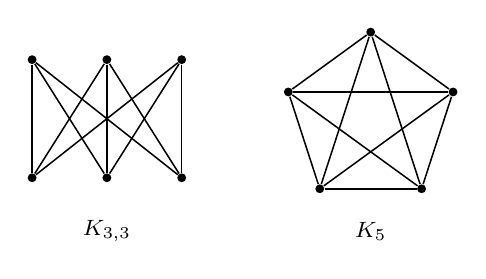
\begin{tikzpicture}[
    font=\footnotesize,
    nodo/.style={circle,fill=black,inner sep=0pt,minimum size=3.2pt},
    arco/.style={line width=0.55pt}]

  %% ============================== K_{3,3} ==================================
  \begin{scope}[shift={(0,0)}]
    \foreach \i in {1,2,3} {
      \node[nodo] (a\i) at ({(\i-1)*0.95}, 1.50) {};
      \node[nodo] (b\i) at ({(\i-1)*0.95}, 0.00) {};
    }
    \foreach \i in {1,2,3}
      \foreach \j in {1,2,3}
        \draw[arco] (a\i) -- (b\j);
    \node at (0.95,-0.68) {$K_{3,3}$};
  \end{scope}

  %% ================================ K_5 ====================================
  \begin{scope}[shift={(4.30,0.75)}]
    \foreach \i/\ang in {1/90, 2/162, 3/234, 4/306, 5/18}
      \node[nodo] (c\i) at (\ang:1.10) {};
    \foreach \i/\j in {1/2,1/3,1/4,1/5,2/3,2/4,2/5,3/4,3/5,4/5}
      \draw[arco] (c\i) -- (c\j);
    \node at (0,-1.43) {$K_5$};
  \end{scope}

\end{tikzpicture}

  \caption{I due minori proibiti del teorema di Wagner: $K_{3,3}$ e $K_5$.}
  \label{fig:minori-esclusi}
\end{figure}

\subsection{Isomorfismo frazionario}

\scan{81}

Se fra due grafi sussiste un isomorfismo frazionario, il raffinamento dei colori
fallisce: i due grafi ricevono la stessa colorazione e WL-1 non riesce a separarli.

\begin{definizione}[Isomorfismo frazionario]
  Siano $G$ e $H$ grafi su $n$ nodi, con matrici di adiacenza $A_G$ e $A_H$. Diciamo che
  $G$ e $H$ sono \emph{frazionariamente isomorfi}, e scriviamo $G \cong_f H$, se esiste
  una matrice doppiamente stocastica $S \in \RR^{n \times n}$ --- cioè con entrate non
  negative e con tutte le righe e tutte le colonne di somma $1$ --- tale che
  \[
    A_G\,S \;=\; S\,A_H .
  \]
\end{definizione}

\begin{osservazione}
  Un isomorfismo vero e proprio è una matrice di \emph{permutazione} $P$ con
  $A_G P = P A_H$; l'isomorfismo frazionario è il rilassamento continuo di quella
  condizione, cioè l'ammissibilità del programma lineare che si ottiene sostituendo le
  matrici di permutazione con quelle doppiamente stocastiche. Il legame con
  Weisfeiler--Leman è esatto, ma vale al primo livello: $G \cong_f H$ se e solo se il
  raffinamento dei colori, cioè WL-1, produce sui due grafi lo stesso multi-insieme di
  colori. È questo il senso della frase qui sopra --- quando l'isomorfismo frazionario
  c'è, la colorazione non ha più nulla su cui fare presa. Ai livelli superiori il
  fallimento non è più garantito: il ciclo $C_6$ e l'unione di due triangoli sono
  frazionariamente isomorfi, essendo entrambi $2$-regolari, eppure WL-2 li distingue,
  perché il suo passo di raffinamento conta i vicini comuni di ogni coppia di vertici
  ($0$ nel ciclo, $1$ per gli archi dei triangoli). Salendo nella gerarchia, la
  controparte di WL-$k$ non è più il programma lineare «nudo», ma il suo livello $k$
  nella gerarchia di Sherali--Adams.
\end{osservazione}

\subsection{La logica con conteggio}

\begin{definizione}[Il frammento $C^{k}$]
  $C^{k}$ è il frammento della logica del prim'ordine in cui si usano
  \begin{itemize}
    \item al più $k$ variabili distinte;
    \item quantificatori esistenziali \emph{con conteggio}
      \[
        \exists^{\ge m} x \; \varphi(x), \qquad m \in \NN,
      \]
      da leggersi «esistono almeno $m$ elementi $x$ per cui vale $\varphi(x)$».
  \end{itemize}
\end{definizione}

\begin{lacuna}
  Nel quaderno, sotto la definizione di $C^{k}$, compare un secondo punto elenco lasciato
  in bianco.
\end{lacuna}

\begin{osservazione}[Cai--Fürer--Immerman, 1992]
  Il punto rimasto in sospeso è quasi certamente l'enunciato che giustifica
  l'introduzione di $C^{k}$: WL-$k$ (nella versione \emph{folklore} adottata qui)
  distingue due grafi $G$ e $H$ se e solo se esiste un enunciato di $C^{k+1}$ vero in uno
  e falso nell'altro. Lo sfasamento di uno è lo stesso già incontrato fra FWL e OWL: è
  OWL-$k$, non FWL-$k$, ad avere il potere distintivo di $C^{k}$. Per $k = 1$ si ritrova
  il caso noto: il raffinamento dei colori ha esattamente il potere distintivo di $C^{2}$,
  la logica a due variabili con conteggio.
\end{osservazione}

\section{Il kernel di Weisfeiler--Leman}

L'algoritmo si può usare anche, al di fuori del problema dell'isomorfismo, come
estrattore di caratteristiche per il machine learning su grafi: si eseguono $r$
iterazioni di Weisfeiler--Leman sul grafo e si conta quante volte compare ciascun colore.
Il vettore dei conteggi $\varphi_r(G)$ è la rappresentazione del grafo, e il kernel è il
prodotto scalare fra le rappresentazioni,
\[
  K(G,H) \;=\; \langle\, \varphi_r(G),\; \varphi_r(H) \,\rangle .
\]

\begin{figure}[H]
  \centering
  % wl-kernel-diamante -- pag. 81
% Il grafo a matita sotto il titolo «WL-kernel»: ciclo di lunghezza 4 con una
% corda, cioe' K_4 privato di un lato (il «diamante»).  I quattro lati del
% quadrato piu' la sola diagonale alto-destra / basso-sinistra: i due vertici
% che essa collega hanno grado 3, gli altri due grado 2.
% Il quadrato e' leggermente irregolare, come nel manoscritto; la corda e'
% tracciata un filo piu' sottile perche' nella scansione ha tratto piu' leggero.
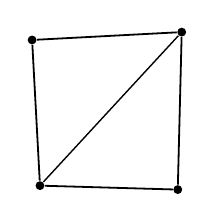
\begin{tikzpicture}[
    font=\footnotesize,
    nodo/.style={circle,fill=black,inner sep=0pt,minimum size=3.2pt},
    arco/.style={line width=0.65pt},
    corda/.style={line width=0.5pt}]

  \node[nodo] (a) at (0.00, 1.85) {};   % alto a sinistra   (grado 2)
  \node[nodo] (b) at (1.90, 1.95) {};   % alto a destra     (grado 3)
  \node[nodo] (c) at (0.10, 0.00) {};   % basso a sinistra  (grado 3)
  \node[nodo] (d) at (1.85,-0.05) {};   % basso a destra    (grado 2)

  \draw[arco]  (a) -- (b);
  \draw[arco]  (a) -- (c);
  \draw[arco]  (b) -- (d);
  \draw[arco]  (c) -- (d);
  \draw[corda] (b) -- (c);

\end{tikzpicture}

  \caption{Il grafo disegnato a matita sotto il titolo «WL-kernel»: un ciclo di lunghezza
  $4$ con una corda, cioè $K_4$ privato di un lato.}
  \label{fig:wl-kernel-diamante}
\end{figure}

\begin{osservazione}
  Annotazione a matita, rimasta a metà: «grafi indistinguibili da WL-$k$
  $\Longrightarrow$ \dots». La conclusione non è stata scritta, ma è obbligata: se
  WL-$k$ non distingue $G$ da $H$, i due grafi hanno lo stesso multi-insieme di colori,
  dunque $\varphi_r(G) = \varphi_r(H)$ e il kernel non li separa. I limiti di
  espressività del test si trasferiscono di peso al kernel, e per lo stesso motivo ---
  l'aggiornamento è quello di Weisfeiler--Leman --- anche alle reti neurali su grafi a
  passaggio di messaggi, che non superano il potere distintivo di WL-1.
\end{osservazione}

% --- Gli appunti si interrompono qui: le pagine successive del quaderno sono bianche.
